% LaTeX Template for Project Report, Version 2.0
% (Abstracted from a Major Project Report at CSED, NIT Calicut but can be
% modified easily to use for other reports also.)
%
% Released under Creative Commons Attribution license (CC-BY)
% Info: http://creativecommons.org/licenses/by/3.0/
%
% Created by: Kartik Singhal
% BTech CSE Batch of 2009-13
% NIT Calicut
% Contact Info: kartiksinghal@gmail.com
%
% It is advisable to learn the basics of LaTeX before using this template.
% A good resource to start with is http://en.wikibooks.org/wiki/LaTeX/
%
% All template fields are marked with a pair of angular brackets e.g. <title here>
% except for the ones defining citation names in ref.tex.
%
% Empty space after chapter/section/subsection titles can be used to insert text.
%
% Just compile this file using pdflatex after making all required changes.

\documentclass[12pt,a4paper]{report}
\usepackage[pdftex]{graphicx} %for embedding images
\usepackage{url} %for proper url entries
\usepackage[bookmarks, colorlinks=false, pdfborder={0 0 0}, pdftitle={<pdf title here>}, pdfauthor={<author's name here>}, pdfsubject={<subject here>}, pdfkeywords={<keywords here>}]{hyperref} %for creating links in the pdf version and other additional pdf attributes, no effect on the printed document
%\usepackage[final]{pdfpages} %for embedding another pdf, remove if not required

\begin{document}
\renewcommand\bibname{References} %Renames "Bibliography" to "References" on ref page

%include other pages
\begin{titlepage}

\begin{center}

\textup{\small {\bf CSU498 Project} \\ Report}\\[0.2in]

% Title
\Large \textbf {<Title here>}\\[0.5in]

       \small \emph{Submitted in partial fulfillment of\\
        the requirements for the award of the degree of}
        \vspace{.2in}

       {\bf Bachelor of Technology \\in\\ Computer Science and Engineering}\\[0.5in]

% Submitted by
\normalsize Submitted by \\
\begin{table}[h]
\centering
\begin{tabular}{lr}\hline \\
Roll No & Names of Students \\ \\ \hline
\\
<Roll no here> & <Name here> \\
<Roll no here> & <Name here> \\ 
<Roll no here> & <Name here> \\ \\ \hline 
\end{tabular}
\end{table}

\vspace{.1in}
Under the guidance of\\
{\textbf{<Guide's name here>}}\\[0.2in]

\vfill

% Bottom of the page

\includegraphics[width=0.18\textwidth]{./nitc-logo}\\[0.1in]
\Large{Department of Computer Science and Engineering}\\
\normalsize
\textsc{National Institute of Technology Calicut}\\
Calicut, Kerala, India -- 673 601 \\
\vspace{0.2cm}
Winter Semester 2013

\end{center}

\end{titlepage}

% \newpage
\thispagestyle{empty}

\begin{center}

\huge{Department of Computer Science and Engineering}\\[0.5cm]
\normalsize
\textsc{National Institute of Technology Calicut}\\[2.0cm]

\emph{\LARGE Certificate}\\[2.5cm]
\end{center}
\normalsize This is to certify that this is a bonafide record of the project presented by the students whose names are given below during <Monsoon/Winter and Year here> in partial fulfilment of the requirements of the degree of Bachelor of Technology in Computer Science and Engineering.\\[1.0cm]

\begin{table}[h]
\centering
\begin{tabular}{lr}
Roll No & Names of Students \\ \\ \hline
\\
<Roll no here> & <Name here> \\ 
<Roll no here> & <Name here> \\
<Roll no here> & <Name here> \\
\end{tabular}
\end{table}

\vfill


% Bottom of the page
\begin{flushright}
<Guide name here>\\
(Project Guide)\\[1.5cm]
<Coordinator name here>\\
(Course Coordinator)\\
\end{flushright}

\begin{flushleft}
Date:
\end{flushleft}

\vspace{2in}
\begin{abstract}
Several $O(n), O(n^2)$ short-cutting heuristics are described which are used in Christofides' algorithm for solving n-city travelling salesman problems whose cost matrix satisfies the triangularity condition. The Christofides' algorithm invovles computation of a shortest spanning tree of the graph G defining the TSP, and finding the minimum cost perfect matching of a certaing induced subgraph of G. 
\end{abstract} 


\pagenumbering{roman} %numbering before main content starts
\tableofcontents
\listoffigures

\newpage
\pagenumbering{arabic} %reset numbering to normal for the main content

\chapter{Goal}

The goal is to find more efficient(in terms of solution cost) short-cutting heuristics which are used in the last step of Christofides' algorithm for finding the TSP tour.

 %objective changed to problem definition
\chapter{Introduction}

\section{Metric space}

A metric $d$ on a set $X$, also called a distance function, is a function
that defines a distance between each pair of elements of the set. A
set with a metric is called a \textbf{metric space}.\\

Formally, $d : X \times X \rightarrow R$ is a metric if it is a function satisfying the following properties $\forall x, y, z \epsilon X$:
\begin{enumerate}
\item{Non-negativity : $d(x, y) \geq 0$}
\item{Indiscernability : $d(x, y) = 0$ iff $x = y$}
\item{Symmetry : $d(x, y) = d(y, x)$}
\item{Subadditivity : $d(x, y) + d(y, z) \geq d(x, z)$}
\end{enumerate}
\section{The Christofides' algorithm}
The Christofides' algorithm is an approximation algorithm for Metric TSP with an approximation ratio of $1.5$. Let G be a graph with $n$ points in the euclidean metric space. Below is a description of the steps involved in the Christofides' algorithm.
\vspace{0.7in}
\subsection{Pseudo code}
\textbf{Algorithm}
\begin{enumerate}
    \item{
        Find an MST of $G$, say $T$.        
    }
    \item {Compute a minimum cost perfect matching, $M$, on the set of odd-degree vertices of $T$.}
    \item {
        Add $M$ to $T$ and obtain an Eulerian multi-graph $H$.
    }
    \item {Find an Euler tour, $E$ of this graph.
    }
    \item {Output the tour that visits vertices of $G$ in order of their first appearance in $E$.}
\end{enumerate}
\begin{figure}[h]
    \centering
    \caption{MST $T$ of $G$}
    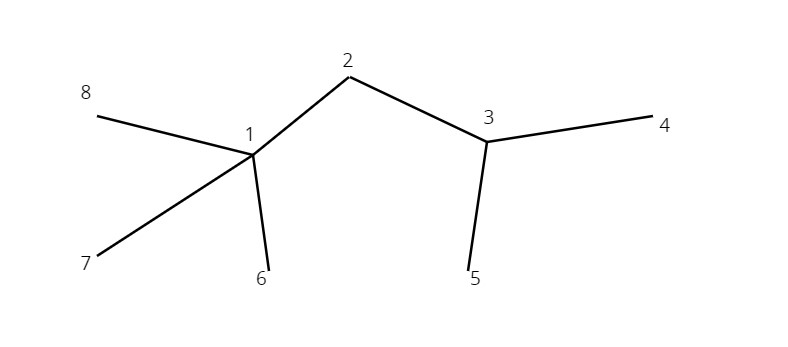
\includegraphics[scale=0.3]{1.jpg}
\end{figure}        
\begin{figure}[h]
    \centering
    \caption{Multi-graph $H$ of $G$}
    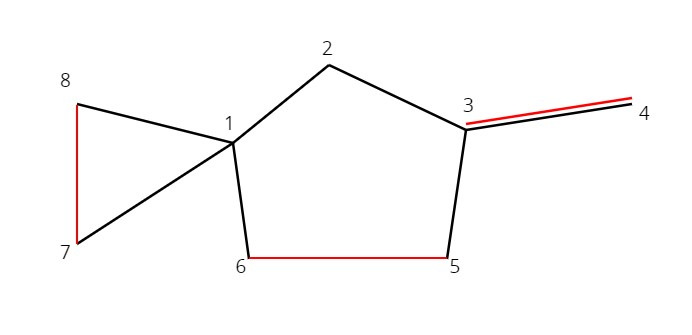
\includegraphics[scale=0.3]{2.jpg}
\end{figure}
\begin{figure}[h]
    \centering
    \caption{Euler tour $E$ of $H$}
    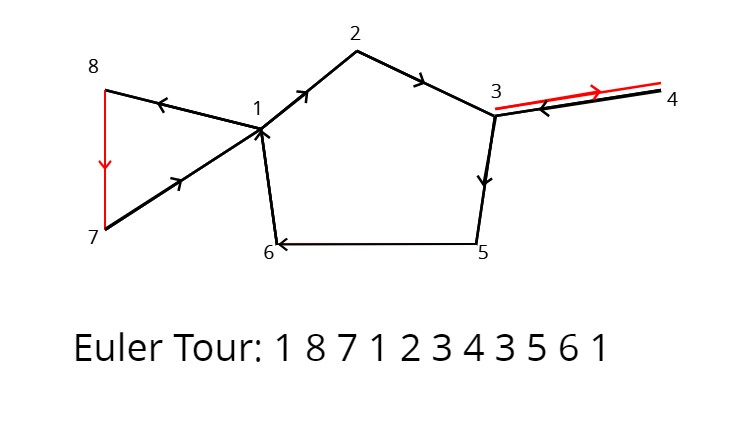
\includegraphics[scale=0.3]{3.jpg}
\end{figure}
\subsection{Time complexity}
\begin{enumerate}
    \item {Creating MST $T$ of $G$ : $O(nlogn)$}
    \item {Finding the minimum cost perfect matching $M$ : $O(n^3)$}
    \item {Creating multi-graph H : $O(n)$}
    \item {Finding Euler tour $E$ in $H$ : $O(n)$}
\end{enumerate}
% some text\cite{citation-1-name-here}, some more texts
% even more text\footnote{<footnote here>}, and even more.
% \section{Motivation}
 %literature survey included in this
\chapter{Work Done}

\section{Short-cutting heuristics}

\subsection{<Sub-section title>}

\subsection{<Sub-section title>}
some text\cite{citation-2-name-here}, some more text
\subsection{<Sub-section title>}

\subsection{<Sub-section title>}

Refer figure \ref{fig:label}.

\begin{figure}[htb]
\centering

\includegraphics[scale=0.3]{./glider} % e.g. insert ./image for image.png in the working directory, adjust scale as necessary
\caption{<Caption here>}
\label{fig:label} % insert suitable label, this is used to refer to a fig from within the text as shown above
\end{figure}

\subsection{<Sub-section title>}


\section{<Section title>}


\chapter{Future Work}

<Future work here>

\chapter{Conclusion}

<Conclusion here>

\cleardoublepage
%\pagebreak
\phantomsection
\addcontentsline{toc}{chapter}{Acknowledgements}
\chapter*{Acknowledgments}
\vspace{1.0in}
<Acknowledgements here>
\\
\\
\\ 
\\
<Name here> \\ 
\\
<Month and Year here>\\
{National Institute of Technology Calicut}\\
\newpage

\cleardoublepage
%\pagebreak
\phantomsection
\addcontentsline{toc}{chapter}{References}
\begin{thebibliography}{99}

\bibitem{citation-1-name-here}Minimum-weight double-tree shortcutting for Metric TSP: Bounding the approximation ratio\\ \url{https://arxiv.org/abs/0711.2399}

\bibitem{citation-2-name-here}Fast minimum-weight double-tree shortcutting for metric TSP: Is the best one good enough?\\ \url{https://dl.acm.org/doi/10.1145/1498698.1594232}

\end{thebibliography}


\end{document}
